\documentclass{standalone}
\usepackage{tikz}
\definecolor{verdeodi}{RGB}{53,113,105} %%%%%%%
\usetikzlibrary{arrows,decorations.markings,plotmarks}

\begin{document}

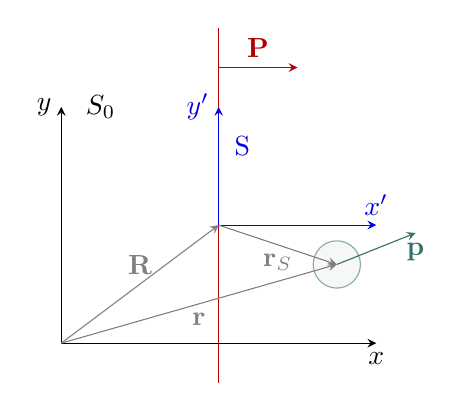
\begin{tikzpicture}

    % MURO
    \draw[red!70!black] (1, -0.5) -- (1, 4);
    \draw[-stealth, red!70!black] (1, 3.5) -- (2, 3.5) node[midway, above]{$\mathbf{P}$};

    % SISTEMA S
    \draw[-stealth] (-1,0) -- (3, 0) node[below]{$x$};
    \draw[-stealth] (-1,0) -- (-1, 3) node[left]{$y$};
    \draw[] (-0.5, 3) node[]{$S_0$};

    % SISTEMA S'
    \draw[-stealth, blue!90!black] (1,1.5) -- (3, 1.5) node[above]{$x'$};
    \draw[-stealth, blue!90!black] (1,1.5) -- (1, 3) node[left]{$y'$};
    \draw[blue!90!black] (1.3, 2.5) node[]{S};

    % BOLA
    \filldraw[color=verdeodi!60, fill=verdeodi!5](2.5, 1) circle (0.3);
    \draw[-stealth, verdeodi] (2.5, 1) -- (3.5, 1.4) node[below]{$\mathbf{p}$};

    % VECTORES POSICION
    \draw[-stealth, gray] (-1,0) -- (2.5, 1) node[midway, below]{$\mathbf{r}$};
    \draw[-stealth, gray] (1,1.5) -- (2.5, 1) node[midway, below]{$\mathbf{r}_S$};
    \draw[-stealth, gray] (-1,0) -- (1,1.5) node[midway, above]{$\mathbf{R}$};
    



\end{tikzpicture}

\end{document}